\documentclass{article}

\usepackage[polish]{babel}
\usepackage[utf8]{inputenc} % Required for inputting international characters
\usepackage[T1]{fontenc} % Output font encoding for international characters
\usepackage{XCharter} % Use the XCharter fonts
\usepackage{graphicx} % graphics


\usepackage{geometry}
\geometry{
	paper=a4paper, % Paper size, change to letterpaper for US letter size
	top=2.5cm, % Top margin
	bottom=3cm, % Bottom margin
	left=2.5cm, % Left margin
	right=2.5cm, % Right margin
	headheight=14pt, % Header height
	footskip=1.5cm, % Space from the bottom margin to the baseline of the footer
	headsep=1.2cm, % Space from the top margin to the baseline of the header
	%showframe, % Uncomment to show how the type block is set on the page
}


\usepackage{listings} % File listings, with syntax highlighting
\lstset{
	basicstyle=\ttfamily, % Typeset listings in monospace font
}

%----------------------------------------------------------------------------------------
%	FILE CONTENTS ENVIRONMENT
%----------------------------------------------------------------------------------------

% Usage:
% \begin{file}[optional filename, defaults to "File"]
%	File contents, for example, with a listings environment
% \end{file}

% \mdfdefinestyle{file}{
% 	innertopmargin=1.6\baselineskip,
% 	innerbottommargin=0.8\baselineskip,
% 	topline=false, bottomline=false,
% 	leftline=false, rightline=false,
% 	leftmargin=2cm,
% 	rightmargin=2cm,
% 	singleextra={%
% 		\draw[fill=black!10!white](P)++(0,-1.2em)rectangle(P-|O);
% 		\node[anchor=north west]
% 		at(P-|O){\ttfamily\mdfilename};
% 		%
% 		\def\l{3em}
% 		\draw(O-|P)++(-\l,0)--++(\l,\l)--(P)--(P-|O)--(O)--cycle;
% 		\draw(O-|P)++(-\l,0)--++(0,\l)--++(\l,0);
% 	},
% 	nobreak,
% }

% Define a custom environment for file contents
\newenvironment{file}[1][File]{ % Set the default filename to "File"
	\medskip
	\newcommand{\mdfilename}{#1}
	\begin{mdframed}[style=file]
}{
	\end{mdframed}
	\medskip
}

\title{WSI} % TODO

\author{Jakub Sobolewski\\ \texttt{300371 Informatyka Sztuczna Inteligencja}} 
\date{\today}

\begin{document}
\maketitle

\section*{Zadanie} % TODO
1) Zaimplementować metodę najszybszego wzrostu/spadku (minimalizacja, spodziewam się stałego współczynnika kroku, jeśli jednak ktoś chce zrobić więcej i zastosować zmienny współczynnik to ma taką możliwość). Gradient wyliczamy numerycznie.

\noindent2) Narysować zachowanie algorytmu (kolejne kroki algorytmu jako strzałki na tle poziomic funkcji celu). Uwaga: w praktycznych zadaniach optymalizacji nie da się narysować funkcji celu ponieważ zadania mają wiele wymiarów (np. 100), oraz koszt wyznaczenia oceny jednego punktu jest duży.

\noindent 3) Zastosować metodę do znalezienia optimum funkcji booth w 2 wymiarach, po czym do znalezienia optimum funkcji o numerach od 1 do 3 z CEC 2017 w 10 wymiarach (na wykresie narysować kroki w wybranych 2 wymiarach z 10). Ograniczenia kostkowe przestrzeni to -100, 100.

\section*{Środowisko}
Python 3.9.7

\section*{Rozwiązanie}
załączone w pliku script.ipynb

\section*{Sprawozdanie}

\subsection*{Funkcja Booth}
Parametry:\\
wymiary: 2\\
$\beta$: 0.000001\\
kroki: 10000\\

\noindent Wartości funkcji celu wynosiły kolejno 632, 324, 20309.
\begin{figure}[!h]
    \centering 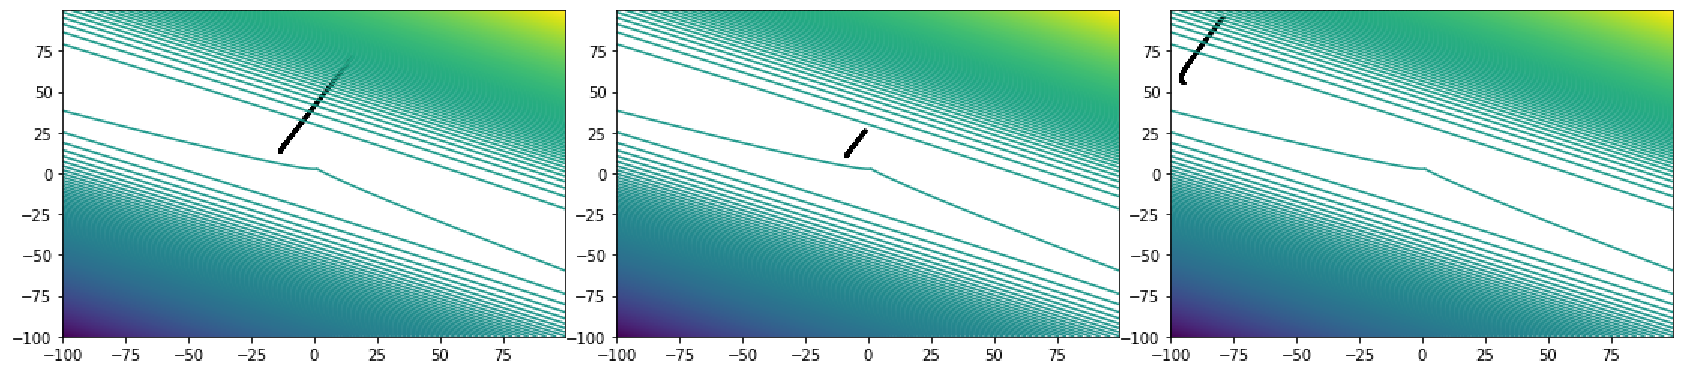
\includegraphics[width=\linewidth]{booth.pdf}
    \caption{Gradienty funkcji Booth}
\end{figure}

\subsection*{Funkcja F1}
Parametry:\\
wymiary: 10\\
$\beta$: 0.00000001\\
kroki: 1000\\

\noindent Wartości funkcji celu wynosiły kolejno 769, 1850, 351.

\begin{figure}[!h]
    \centering 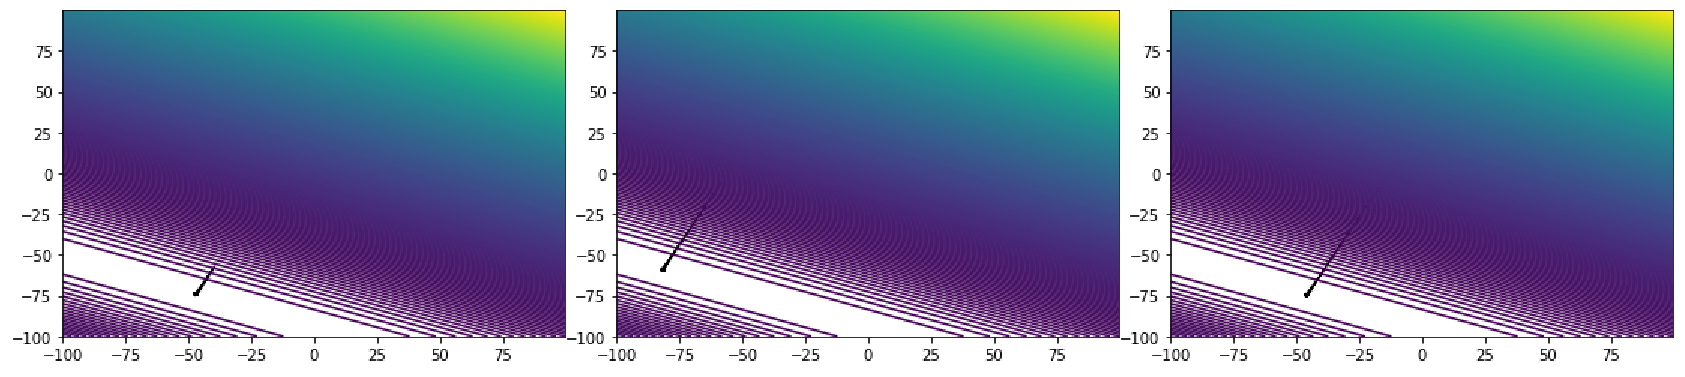
\includegraphics[width=\linewidth]{f1.pdf}
    \caption{Gradienty funkcji F1}
\end{figure}

\subsection*{Funkcja F2}
Parametry:\\
wymiary: 10 i 2\\
$\beta$: 0.00000001\\
kroki: 1000\\

\noindent W 2 wymiarach udaje się znaleźć optimum, przy większej liczbie wymiarów, ciężko znaleźć dobrą beta, raz jest za duża i problem nie jest zbieżny a raz za wolno się uczy.

\noindent Wartości funkcji celu wynosiły kolejno 200 (2 wymiary), 243428399153146 (10 wymiarów), 13074639241675 (10 wymiarów).
\begin{figure}[!h]
    \centering 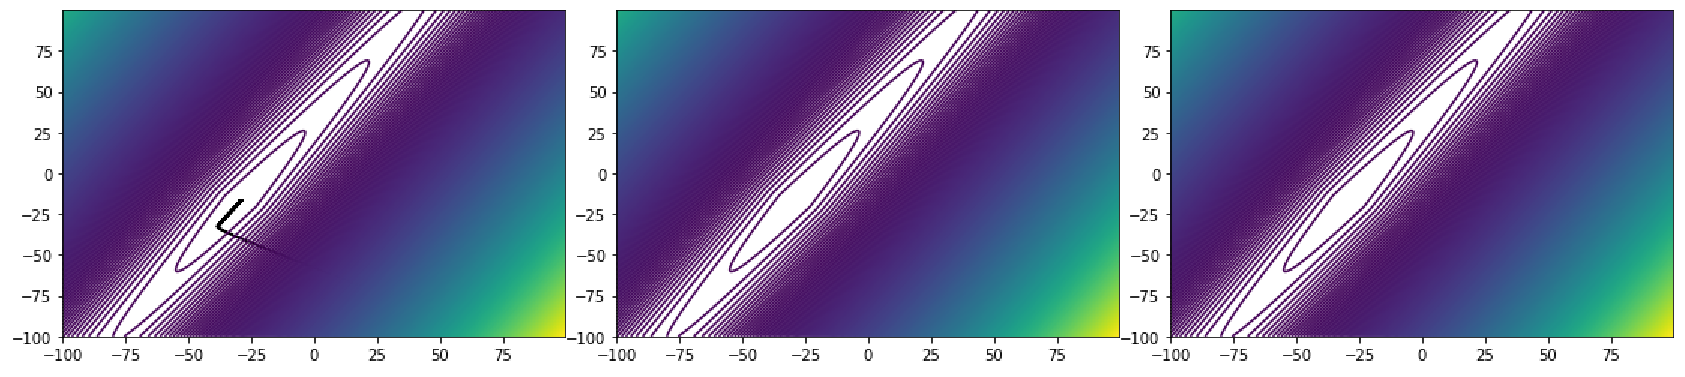
\includegraphics[width=\linewidth]{f2.pdf}
    \caption{Gradienty funkcji F2}
\end{figure}


\subsection*{Funkcja F3}
Parametry:\\
wymiary: 10\\
$\beta$: 0.00000001\\
kroki: 1000, 10000\\

\noindent Wartości funkcji celu wynosiły kolejno 64579 (1000 kroków), 43858 (10000 kroków), 25628 (10000 kroków).

\begin{figure}[!h]
    \centering 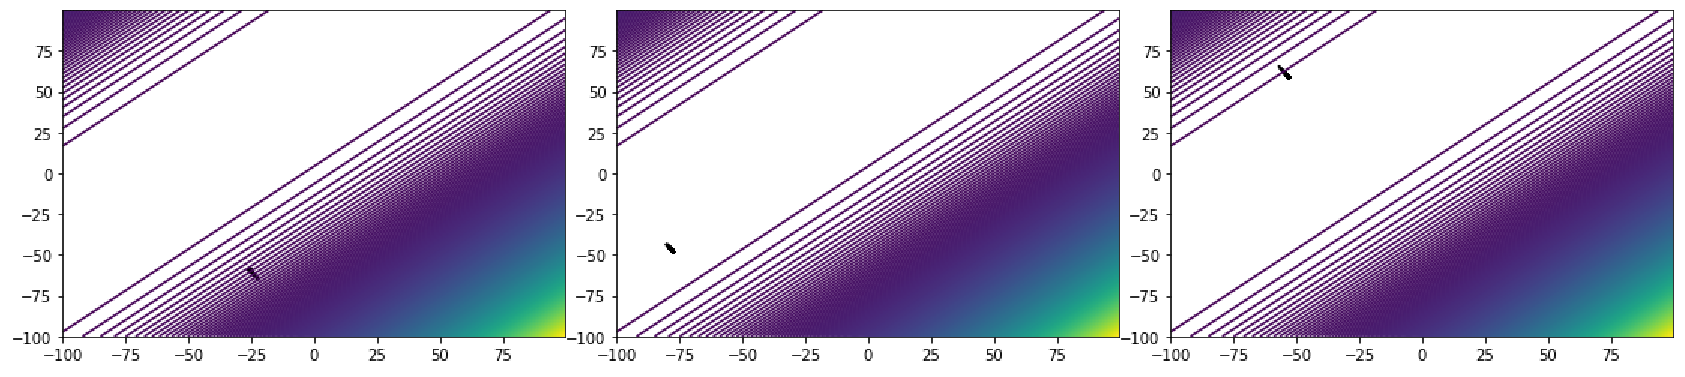
\includegraphics[width=\linewidth]{f3.pdf}
    \caption{Gradienty funkcji F3}
\end{figure}

\section*{Pytania}
\noindent\textbf{Jak wartość parametru beta wpływa na szybkość dojścia do optimum i zachowanie algorytmu?}\\
Za mała beta powoduje dużą ilość iteracji potrzebnych do osiągnięcia optimum. za duża beta powoduje niestabilność, czyli $f(x) = \infty$ lub wartość funkcji zmienia się skokowo w górę i w dół.\\

\noindent\textbf{Zalety/wady algorytmu?}\\
Zalety: prosty, zwraca rozwiązanie optymalne (o ile nie utknie w minimum lokalnym).\\
Wady: nie działa dla nieznanej funkcji (wtedy trzeba inaczej gradient liczyć).\\

\noindent\textbf{Wnioski}\\
Każda funkcja zachowuje się inaczej, jednych łatwiej znaleźć optimum innych trudniej, dobranie hiperparametów ma kluczowe znaczenie w szukaniu optymalnego rozwiązania.

\end{document}


